% copied from the thesis chapter on fairness (content/fairness/fairness.tex, lines 779-1003)
\begin{figure}[!htbp]
  \begin{center}
      
    \begin{subfigure}[t]{0.3\textwidth}
        \begin{center}
            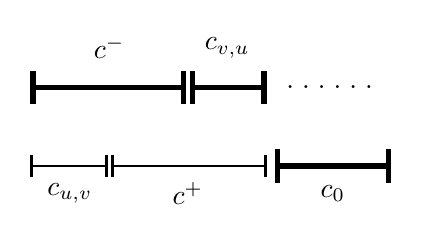
\begin{tikzpicture}

  \draw[line width=2, |-|]
  ({0.5}, 2.5) -- ({2.48}, 2.5) node[anchor=north west] {};
  \node at ({1.5}, 3) {$c^-$};
  \draw[line width=1, |-|]
  ({1.52}, 1.5) -- ({3.5}, 1.5) node[anchor=north west] {};
  \node at ({2.5},1.15) {$c^+$};
  
  \draw[line width=1, |-|]
  ({.5}, 1.5) -- ({1.48}, 1.5) node[anchor=north west] {};
  \node at ({1.},1.15) {$c_{u,v}$};
  \draw[line width=2, |-|]
  ({2.52}, 2.5) -- ({3.5}, 2.5) node[anchor=north west] {};
  \node at ({3.},3) {$c_{v,u}$};

  % the job of $c_0$, containing the jobs of the clients not mentioned above
  \draw[line width=2, |-|]
  ({3.6}, 1.5) -- ({5.08}, 1.5) node[anchor=north west] {};
  \node at ({4.34}, 1.15) {$c_0$};
  \node at ({4.3}, 3.) {}; % {$c$};
  \foreach \x in
    {
        1,2,3,4,5,6
    }
    {
        \node at ({3.6+\x*0.2}, 2.5) {$.$};
    }
  
            \end{tikzpicture}
        \end{center}
        \caption{$v\in I , u \notin I$.}
        \end{subfigure}
        \hspace{.3cm}
           \begin{subfigure}[t]{0.3\textwidth}
        \begin{center}
            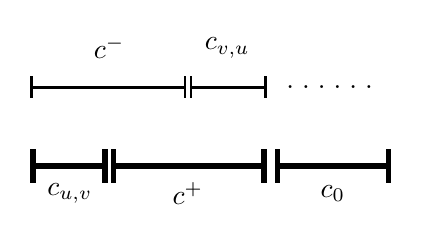
\begin{tikzpicture}

  \draw[line width=1, |-|]
  ({0.5}, 2.5) -- ({2.48}, 2.5) node[anchor=north west] {};
  \node at ({1.5}, 3) {$c^-$};
  \draw[line width=2, |-|]
  ({1.52}, 1.5) -- ({3.5}, 1.5) node[anchor=north west] {};
  \node at ({2.5},1.15) {$c^+$};
  
  \draw[line width=2, |-|]
  ({.5}, 1.5) -- ({1.48}, 1.5) node[anchor=north west] {};
  \node at ({1.},1.15) {$c_{u,v}$};
  \draw[line width=1, |-|]
  ({2.52}, 2.5) -- ({3.5}, 2.5) node[anchor=north west] {};
  \node at ({3.},3) {$c_{v,u}$};

  % the job of $c_0$, containing the jobs of the clients not mentioned above
  \draw[line width=2, |-|]
  ({3.6}, 1.5) -- ({5.08}, 1.5) node[anchor=north west] {};
  \node at ({4.34}, 1.15) {$c_0$};
  \node at ({4.3}, 3.) {}; % {$c$};
  \foreach \x in
    {
        1,2,3,4,5,6
    }
    {
        \node at ({3.6+\x*0.2}, 2.5) {$.$};
    }
  
            \end{tikzpicture}
        \end{center}
        \caption{$ v \notin I, u\in I$.}
        \end{subfigure}      
        \hspace{.3cm}
        \begin{subfigure}[t]{0.3\textwidth}
        \begin{center}
            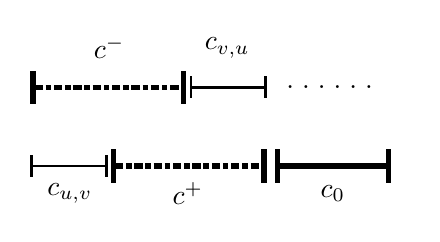
\begin{tikzpicture}

  \draw[line width=2, densely dash dot, |-|]
  ({0.5}, 2.5) -- ({2.48}, 2.5) node[anchor=north west] {};
  \node at ({1.5}, 3) {$c^-$};
  \draw[line width=2, densely dash dot, |-|]
  ({1.52}, 1.5) -- ({3.5}, 1.5) node[anchor=north west] {};
  \node at ({2.5},1.15) {$c^+$};
  
  \draw[line width=1, |-|]
  ({.5}, 1.5) -- ({1.48}, 1.5) node[anchor=north west] {};
  \node at ({1.},1.15) {$c_{u,v}$};
  \draw[line width=1, |-|]
  ({2.52}, 2.5) -- ({3.5}, 2.5) node[anchor=north west] {};
  \node at ({3.},3) {$c_{v,u}$};

  % the job of $c_0$, containing the jobs of the clients not mentioned above
  \draw[line width=2, |-|]
  ({3.6}, 1.5) -- ({5.08}, 1.5) node[anchor=north west] {};
  \node at ({4.34}, 1.15) {$c_0$};
  \node at ({4.3}, 3.) {}; % {$c$};
  \foreach \x in
    {
        1,2,3,4,5,6
    }
    {
        \node at ({3.6+\x*0.2}, 2.5) {$.$};
    }
  
\end{tikzpicture}
\end{center}
\caption{$u,v \notin I$: schedule either $c^+$ or\ $c^-$ such that $c^+$ and $c^-$ are satisfied. }
\end{subfigure}
  \end{center}
%   \begin{center}
      
%     \begin{subfigure}[t]{0.3\textwidth}
%         \begin{center}
%             \begin{tikzpicture}

%     \draw[line width=2, |-|]
%   ({0.48}, 1.5) -- ({-1.}, 1.5) node[anchor=north west] {};
%   \node at (({-.25}, 1.15) {$c_0$};
%   \node at ({-0.25}, 3.) {}; % {$c$};
%   \foreach \x in
%     {
%         1,2,3,4,5,6
%     }
%     {
%         \node at ({-1+\x*0.2}, 2.5) {$.$};
%     }
  
  
%   \draw[line width=2, |-|]
%   ({0.5}, 2.5) -- ({2.48}, 2.5) node[anchor=north west] {};
%   \node at (({1.5}, 3) {$c^-$};
%   \draw[line width=1, |-|]
%   ({1.52}, 1.5) -- ({3.5}, 1.5) node[anchor=north west] {};
%   \node at ({2.5},1.15) {$c^+$};
  
%   \draw[line width=1, |-|]
%   ({.5}, 1.5) -- ({1.48}, 1.5) node[anchor=north west] {};
%   \node at ({1.},1.15) {$c_{u,v}$};
%   \draw[line width=2, |-|]
%   ({2.52}, 2.5) -- ({3.5}, 2.5) node[anchor=north west] {};
%   \node at ({3.},3) {$c_{v,u}$};
  
%             \end{tikzpicture}
%         \end{center}
%         \caption{$v\in I , u \notin I$.}
%         \end{subfigure}
%         \hspace{.3cm}
%            \begin{subfigure}[t]{0.3\textwidth}
%         \begin{center}
%             \begin{tikzpicture}

%              \draw[line width=2, |-|]
%   ({0.48}, 1.5) -- ({-1.}, 1.5) node[anchor=north west] {};
%   \node at (({-.25}, 1.15) {$c_0$};
%   \node at ({-0.25}, 3.) {}; % {$c$};
%   \foreach \x in
%     {
%         1,2,3,4,5,6
%     }
%     {
%         \node at ({-1+\x*0.2}, 2.5) {$.$};
%     }
                
%   \draw[line width=1, |-|]
%   ({0.5}, 2.5) -- ({2.48}, 2.5) node[anchor=north west] {};
%   \node at (({1.5}, 3) {$c^-$};
%   \draw[line width=2, |-|]
%   ({1.52}, 1.5) -- ({3.5}, 1.5) node[anchor=north west] {};
%   \node at ({2.5},1.15) {$c^+$};
  
%   \draw[line width=2, |-|]
%   ({.5}, 1.5) -- ({1.48}, 1.5) node[anchor=north west] {};
%   \node at ({1.},1.15) {$c_{u,v}$};
%   \draw[line width=1, |-|]
%   ({2.52}, 2.5) -- ({3.5}, 2.5) node[anchor=north west] {};
%   \node at ({3.},3) {$c_{v,u}$};
  
%             \end{tikzpicture}
%         \end{center}
%         \caption{$ v \notin I, u\in I$.}
%         \end{subfigure}      
%         \hspace{.3cm}
%         \begin{subfigure}[t]{0.3\textwidth}
%         \begin{center}
%             \begin{tikzpicture}

%              \draw[line width=2, |-|]
%   ({0.48}, 1.5) -- ({-1.}, 1.5) node[anchor=north west] {};
%   \node at (({-.25}, 1.15) {$c_0$};
%  \node at ({-0.25}, 3.) {}; % {$c$};
%   \foreach \x in
%     {
%         1,2,3,4,5,6
%     }
%     {
%         \node at ({-1+\x*0.2}, 2.5) {$.$};
%     }
                
%   \draw[line width=2, densely dash dot, |-|]
%   ({0.5}, 2.5) -- ({2.48}, 2.5) node[anchor=north west] {};
%   \node at (({1.5}, 3) {$c^-$};
%   \draw[line width=2, densely dash dot, |-|]
%   ({1.52}, 1.5) -- ({3.5}, 1.5) node[anchor=north west] {};
%   \node at ({2.5},1.15) {$c^+$};
  
%   \draw[line width=1, |-|]
%   ({.5}, 1.5) -- ({1.48}, 1.5) node[anchor=north west] {};
%   \node at ({1.},1.15) {$c_{u,v}$};
%   \draw[line width=1, |-|]
%   ({2.52}, 2.5) -- ({3.5}, 2.5) node[anchor=north west] {};
%   \node at ({3.},3) {$c_{v,u}$};
  
% \end{tikzpicture}
% \end{center}
% \caption{$u,v \notin I$: schedule either $c^+$ or\ $c^-$ such that $c^+$ and $c^-$ are satisfied. }
% \end{subfigure}
%   \end{center}

\caption{
The three possible cases on an \textit{edge day} (with $v\in V_i$ and $u\in V_j$ with $i<j$) given a multicolored independent set $I$. We mark the jobs which are included in a schedule constructed from $I$ in \textbf{bold}, and the jobs which do not appear in the figure are pairwise disjoint and are all contained in the job of client $c_0$ (but are not scheduled). There are $\ell \cdot r$ days of types (a) and~(b), as~$|E|$ is even we can freely use (c) days to ensure both $c^+$ and $c^-$ are satisfied.  
}
\label{fig:edgeday}
\end{figure}
